\chapter{Literature review}\label{cap:literature}

This chapter provides an overview of the current state of literature on a variety of subjects related to the thesis.
Its main goals are to provide the reader with context for the research described here and to highlight the research gap that the work tries to address.
Where appropriate, references for in-depth materials on topics that are out of scope of this work are provided.

\section{Remote sensing for forestry applications}

As was mentioned in the introduction, remote sensing is widely used for extending labor-intensive and time-consuming manual forest inventories.
This section provides examples of various remote sensing techniques used in various forestry applications, before going in more detail into specifically \gls{uav} \gls{lidar} and \gls{rgb}, which are the focus of the described framework.

\citet{hansenAssessingForestNonForest2020} explore the usage of C-band \gls{sar} data from the Sentinel-1 mission for binary land use classification into forest/non-forest using a collection of classic machine learning classifiers.
\gls{sar} is an active sensor, making it independent on external conditions and observation time, and it penetrates cloud cover, making it very reliable during almost any weather.
They report accuracies from 80\% in the worst case to the 93\% in the best case, depending on the area of application.

\citet{ferrariFusingSentinel1Sentinel22023} use Fully Convolutional Networks \citep{longFullyConvolutionalNetworks2015} for fusion of multispectral Sentinel-2 and C-band \gls{sar} Sentinel-1 data for clear-cut logging detection in the presence of clouds, which limit the use of optical-only approaches and are very common in tropical areas.
They show that fusion performs better than single-modality variant for pixels obscured by clouds.
This combination of active \gls{sar} and passive multispectral data is very common, as the sensors compliment each other nicely, similarly to laser scanning and orthophotos.

\citet{sinica-sinavskisForestStandVolume2022} combine \gls{lidar} point clouds with Sentinel-2 images to predict timber volume on a stand level.
They use an unusual approach, using Sentinel-2 images for species detection by clustering, \gls{lidar} point clouds for estimating tree counts and average tree heights, and combining them into two variables used to fit the final regression models.
The reported relative \gls{rmse} values are 14-22\%, with errors larger for deciduous tree species.

\gls{lidar} has been used for forestry applications for a long time, with publications on the topic dating back 40 years.
\citet{nelsonDeterminingForestCanopy1984} is one of the earliest studies that explores usage of airborne \gls{lidar} for measuring forest canopy profiles and estimating tree heights and canopy closure (a measure of forest canopy coverage that indicates what proportion of the sky is obscured by the tree crowns when viewed from the ground).
\citet{nilssonEstimationTreeHeights1996} is a study looking into tree height and timber volume estimation using airborne \gls{lidar} across a range of point densities and seasons on a coniferous forest stand.
\citet{naessetDeterminationMeanTree1997} and \citet{naessetEstimatingTimberVolume1997} are studies exploring the use of airborne \gls{lidar} for estimating mean tree height and timber volume, suggesting the ways to correct the systematic underestimation of height and showing how regression on \gls{lidar}-derived metrics can predict volume.
\citet{carson2004lidar} offers an overview of some of the applications and approaches and a summary of contemporary state-of-the-art.

\section{Machine learning and deep learning on point clouds}\label{sec-ml-dl}

The reader is assumed to be familiar with general concepts of machine learning and deep learning.
For an introduction or a refresher, one of the best resources is \citet{goodfellowDeepLearning2016}.
For a more detailed exploration, \citet{wangRecentAdvancesDeep2020} offer a selection of papers on topics relevant to modern deep learning techniques.
As point clouds are a less well-known modality in machine learning and deep learning, the reader is also referred to \citet{belloReviewDeepLearning2020} and \citet{guoDeepLearning3D2021}, offering detailed reviews of the deep learning approaches used in various problems related to processing point clouds.
Figure~\ref{fig-deep-learnin-on-point-clouds} is a high-level taxonomy of these approaches.
Two main groups are structured grid-based, which rely on transformation of point clouds into regular structures that are then processed by 2D or 3D convolutional neural networks, and raw point cloud based, which consume point clouds directly.
There are also more modern and powerful approaches, like the transformer-based Point Transformer \citep{zhaoPointTransformer2021,wuPointTransformerV22022,wuPointTransformerV32024} that utilizes the power of the attention mechanisms that dominates natural language applications and performs well in computer vision.
Another novel addition is PointMamba \citep{liangPointMambaSimpleState2024}, another architecture popularized in the natural language processing domain, aiming to improve on the transformer architecture by using a less computationally complex algorithm called state space model.
The section is focused on providing a very short overview of these topics as it relates to the framework that is the focus of the thesis.

\begin{figure}
\centering{
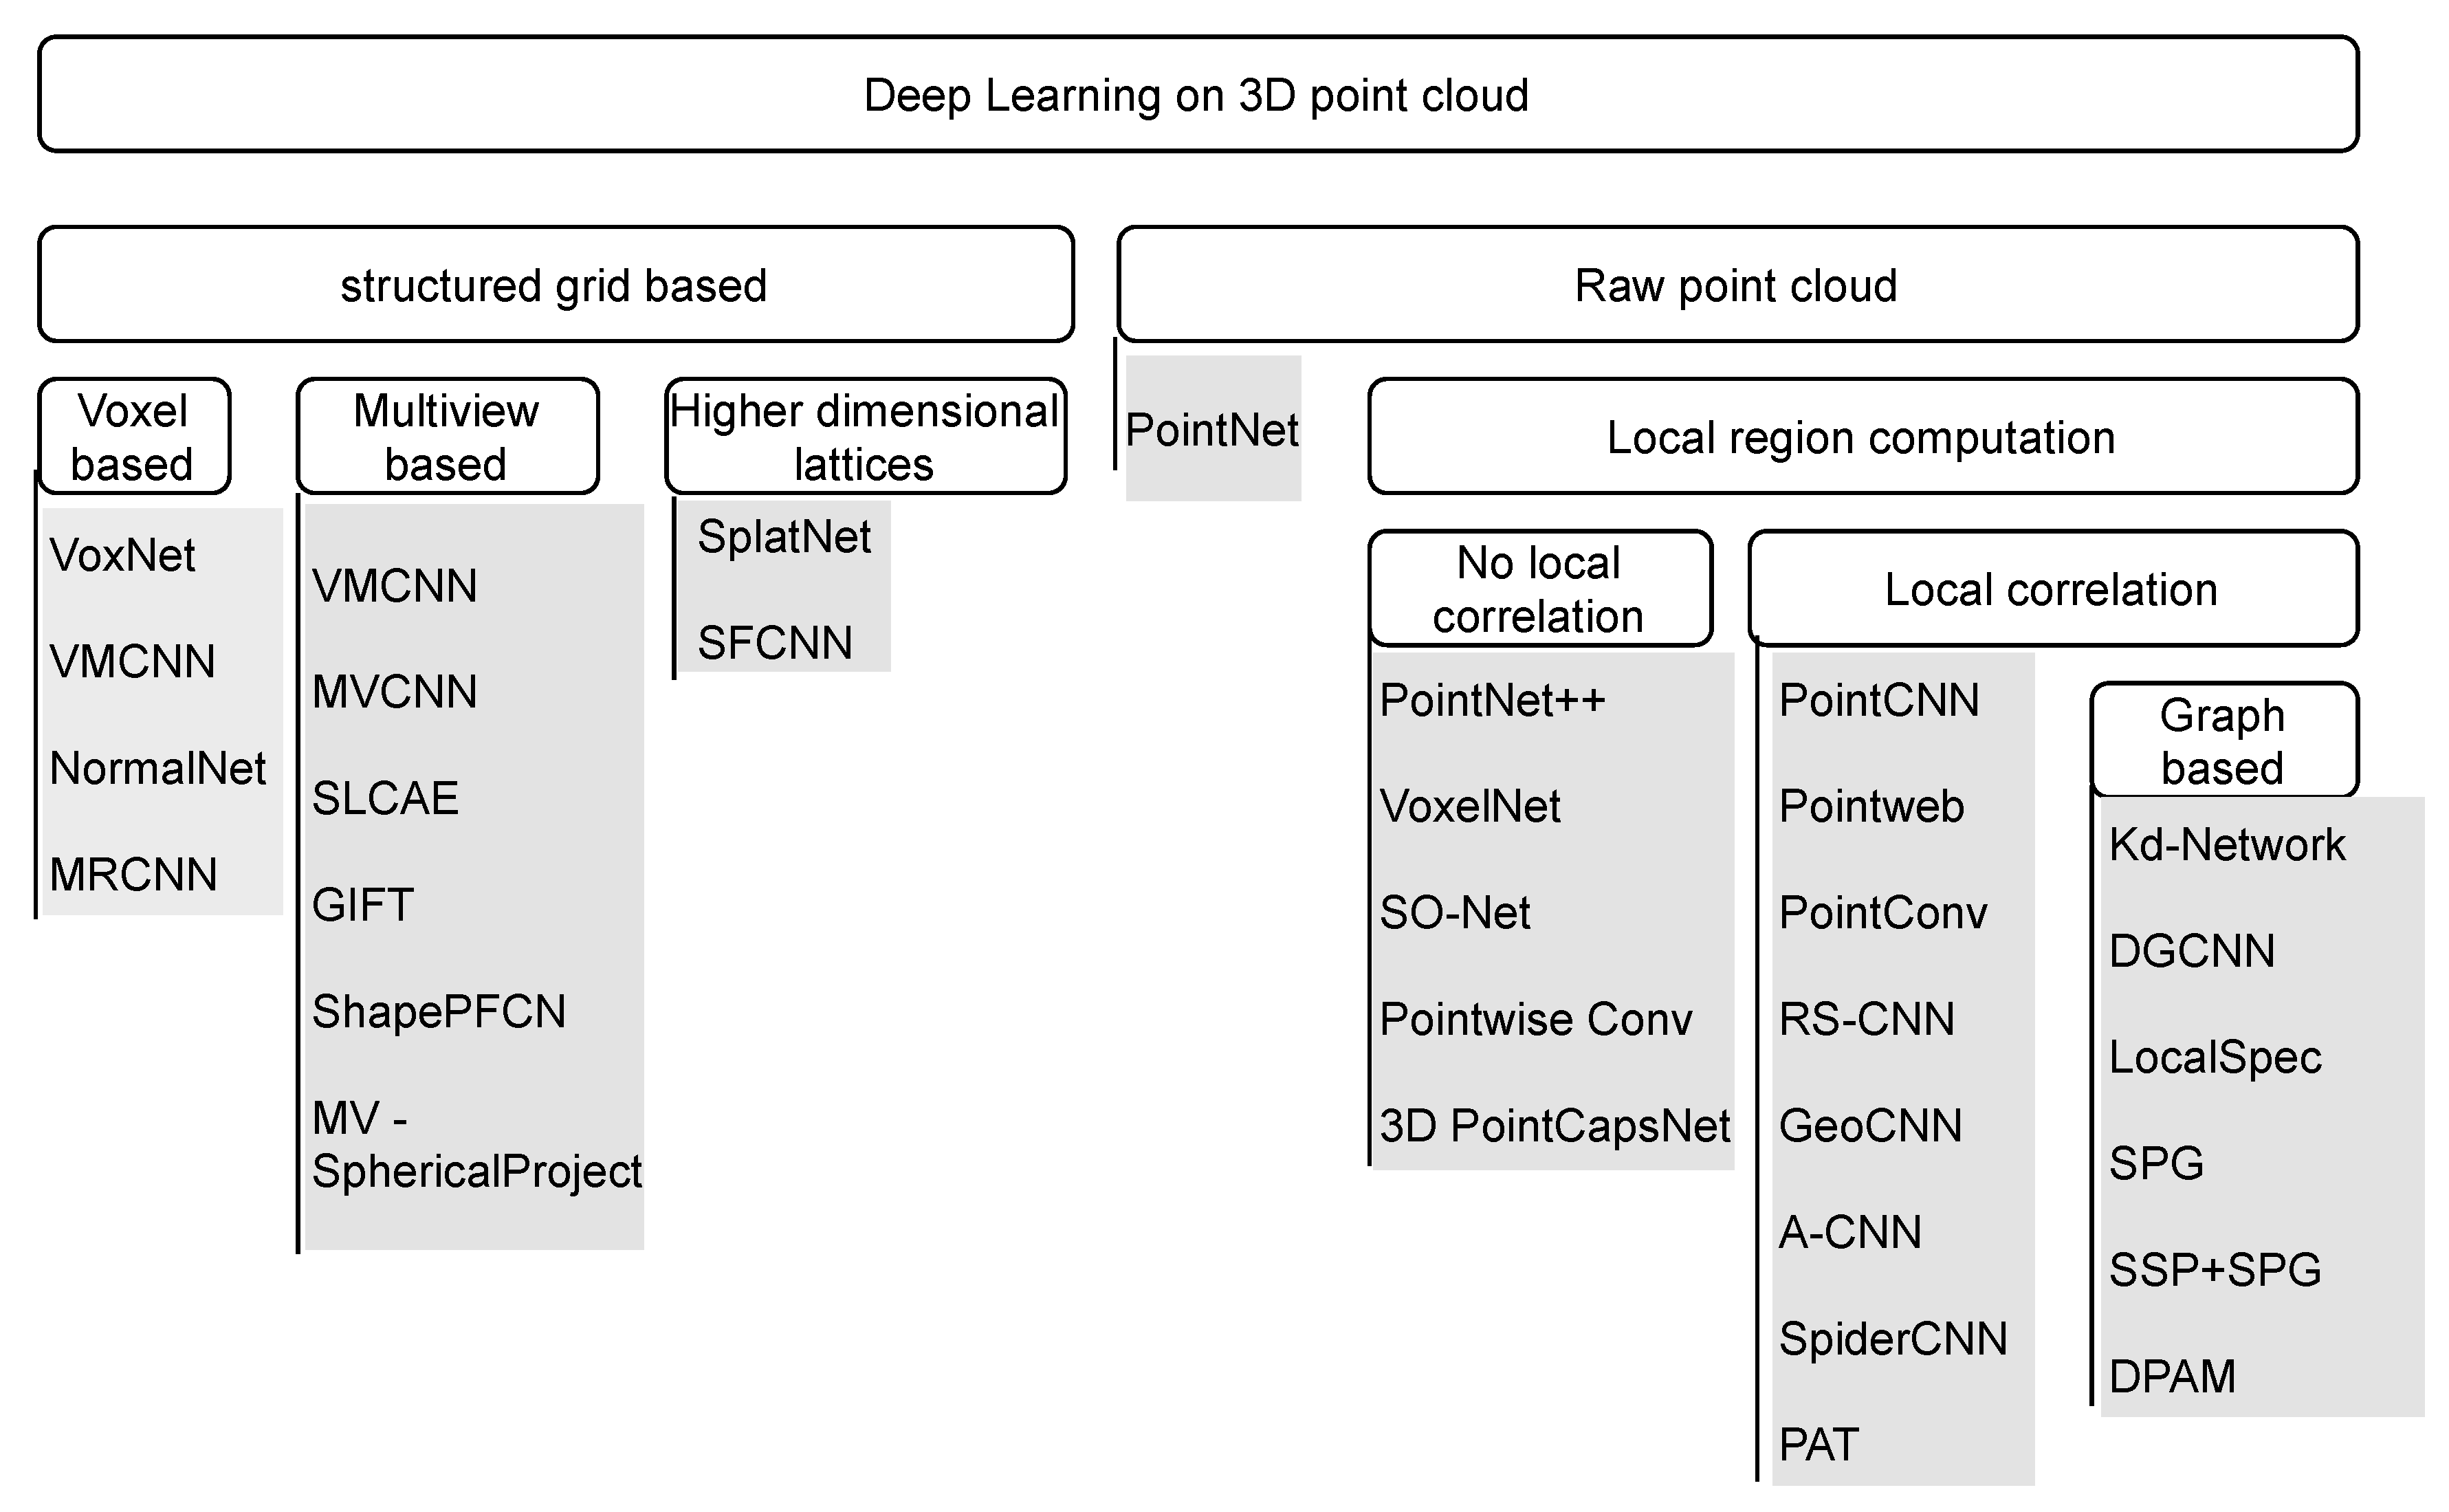
\includegraphics[width=\textwidth]{../images/deep_learning_on_point_clouds.png}
}
\caption[Taxonomy of deep learning methods for point clouds.]{\label{fig-deep-learnin-on-point-clouds}A high-level taxonomy
of deep learning approaches for point clouds. Figure from Bello et al.
(2020)}
\end{figure}

Classic machine learning approaches rely on feature engineering: manual preparation of features used as inputs for models based on domain expertise and various feature selection techniques.
Two main groups of tasks are per-point predictions, which is in many ways similar to the task of semantic segmentation of images, that requires per-point features, and per-cloud predictions that either process entire point clouds or individual segments, separated by some preprocessing routine.
\citet{weinmannFeatureRelevanceAssessment2013} show that careful selection of features is crucial for accurate and efficient semantic interpretation of point cloud data: a shotgun approach of using many simple features without much consideration results in worse performance than a surgical approach of using a few carefully selected ones.
They also provide definitions of some of the most used manual features that aim to describe the 3D structure of point sets.
The features are based on combinations of eigenvalues of local covariance matrices of coordinate vectors of a set of points.
They can be calculated on a per-point basis by using fixed-size or nearest-neighbor neighborhoods, or for whole segments of point clouds.
The used features were originally introduced by \citet{westContextdrivenAutomatedTarget2004}, \citet{paulyEfficientSimplificationPointsampled2002}, and \citet{malletRelevanceAssessmentFullwaveform2011}, and include linearity, planarity, and scatter, aiming to indicate the presence of a linear, planar, or volumetric structures, and also omnivariance, anisotropy, eigentropy, the sum of eigenvalues, and curvature.
The formulas for the features are provided in Section~\ref{sec-training-tree-processors}, where they are used for training parameter prediction models for segmented trees.
Simpler features, that are especially often used in area-based approach, include various statistics describing height and reflection intensity distributions of points, like percentages of points above mean height, deciles of height, cumulative percentages of points below height deciles, and others.
Since many \gls{lidar} sensors can record multiple reflections from a single pulse, features that use the reflection numbers are also often used, i.e., relative return number and total number of returns.

Point clouds are by their nature irregular, and non-uniform point densities across the cloud often become a problem for both manual feature creation and representation learning as part of a deep learning model.
Many researches explore ways to handle this non-uniformity.
For example, \citet{ozdemirDeepLearningFramework2021} proposes a framework for semantic segmentation of photogrammetric point clouds in urban environments, the key components of which are voxel-grid filtering-based downsampling for equalizing the point density across the cloud, manual addition of geometric features in a nearest-neighbor neighborhood, and processing the result with a convolutional network for assigning labels to each point, followed by a post-processing step to upscale the labels back to original point cloud size.

The first deep learning model to work directly on point clouds without constructing any intermediate representation that can be processed by convolutional models is the PointNet introduced by \citet{qiPointNet2017}.
Figure~\ref{fig-pointnet-architecture} shows its architecture.
A critical aspect of any model that aims to operate directly on point clouds is permutation invariance, as point clouds are unordered sets, and shuffling the points does not change the point cloud semantically.
PointNet achieves that invariance by using a combination of shared \glspl{mlp} to process point coordinates and features and max pooling for construction of global feature vector.
That feature vector can then be used directly for point cloud classification tasks, or concatenated with point features and processed further by shared \glspl{mlp} for per-point predictions.

\begin{figure}
\centering{
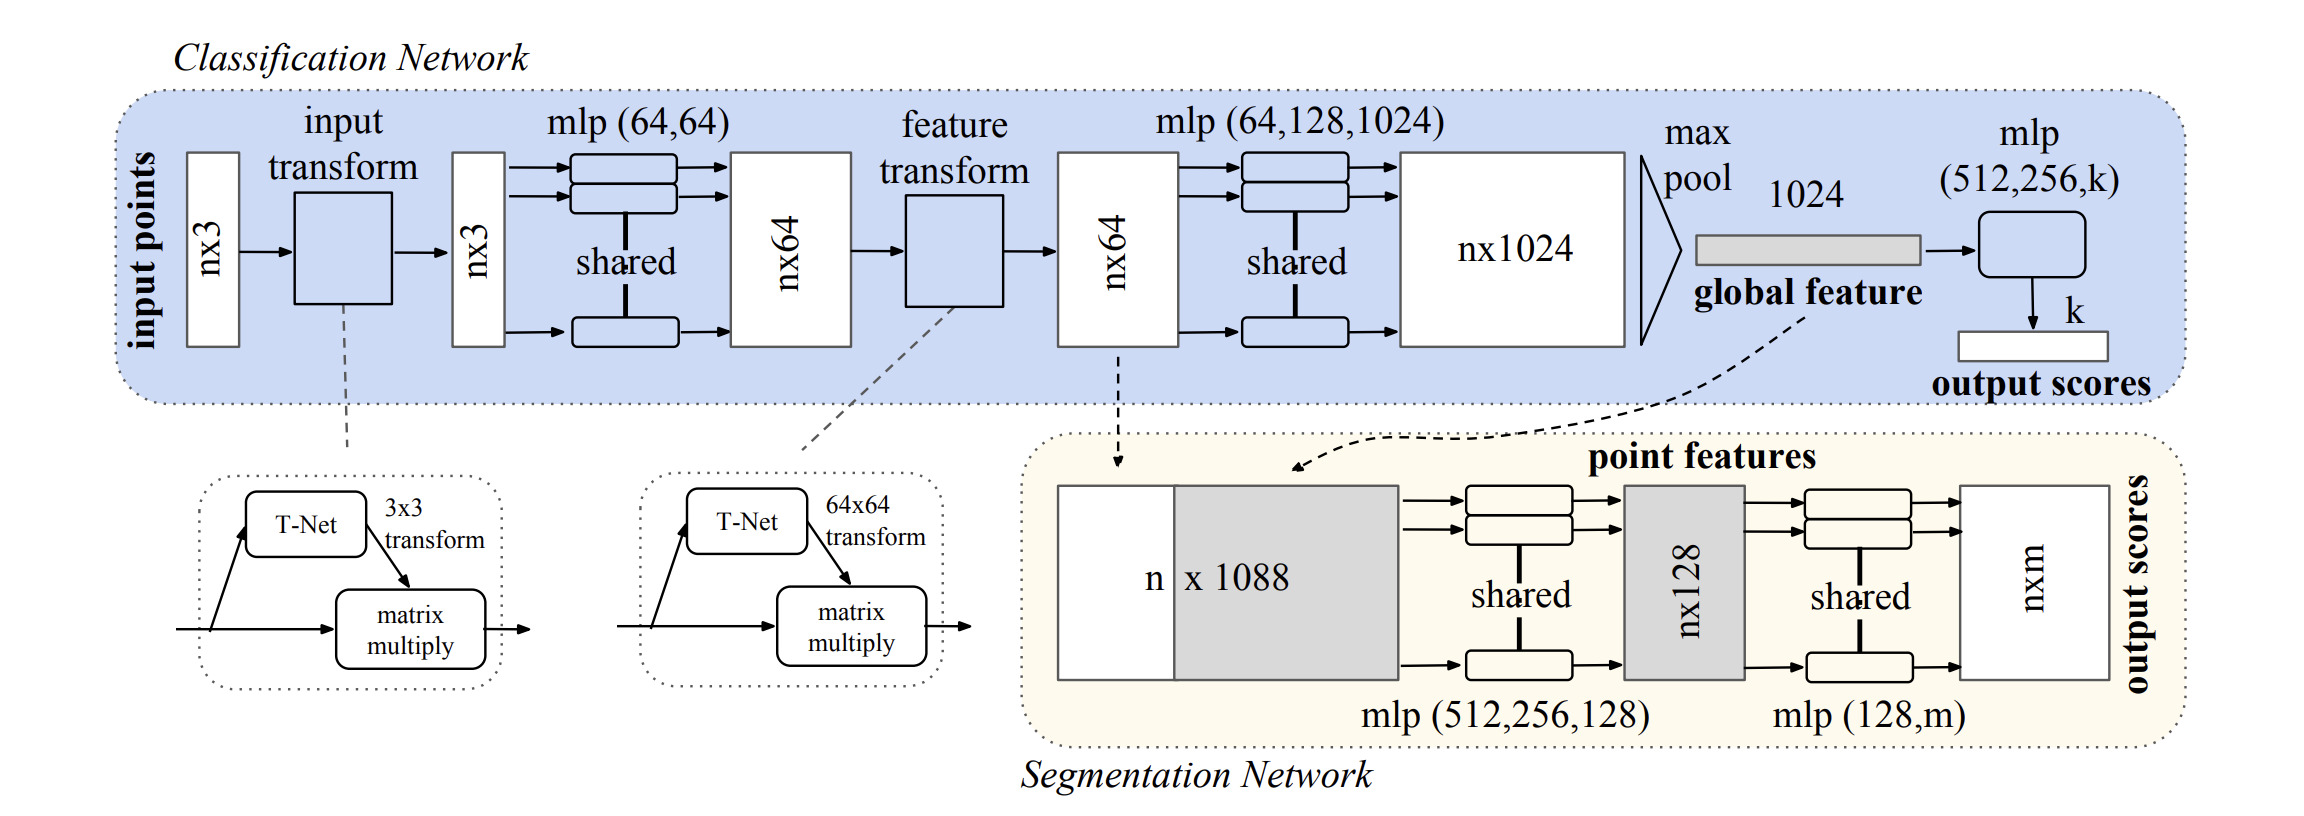
\includegraphics[width=\textwidth]{../images/pointnet_architecture.jpg}
}
\caption[PointNet architecture]{\label{fig-pointnet-architecture}PointNet architecture. Figure
from (Qi, Su, et al. 2017)}
\end{figure}

\citet{qiPointNetPlusPlus2017} introduces PointNet++, aimed to address the main drawbacks of the original PointNet model, namely the use of only two scales for context encoding – per-point and global, which limits the ability of the model to respond to local structures and fine patterns and thus work in complex scenes.
To address this, PointNet++ uses a hierarchical architecture that applies PointNet recursively on nested subsets of the original point set, allowing to learn features on multiple increasing scales.
To achieve that, network uses stacked set abstraction layers, that first sample a subset of the point cloud using farthest point sampling – an algorithm aimed to create representative subsets even for point clouds with uneven point density that selects the next point by maximizing its distance to already selected set – then constructs a neighborhood around each selected point using either fixed distance or fixed number of neighbors, and finally applies PointNet to each neighborhood to reduce into a feature vector for the sampled point.
Then, similar to the original PointNet, the subset can be further reduced to a final global feature vector used for point clouds classification, or passed to an upscaling branch with skip-connections and k-nearest neighbors interpolation to upscale the features to the original point cloud coordinates.
The architecture is visualized in Figure~\ref{fig-pointnet2-architecture}.

\begin{figure}
\centering{
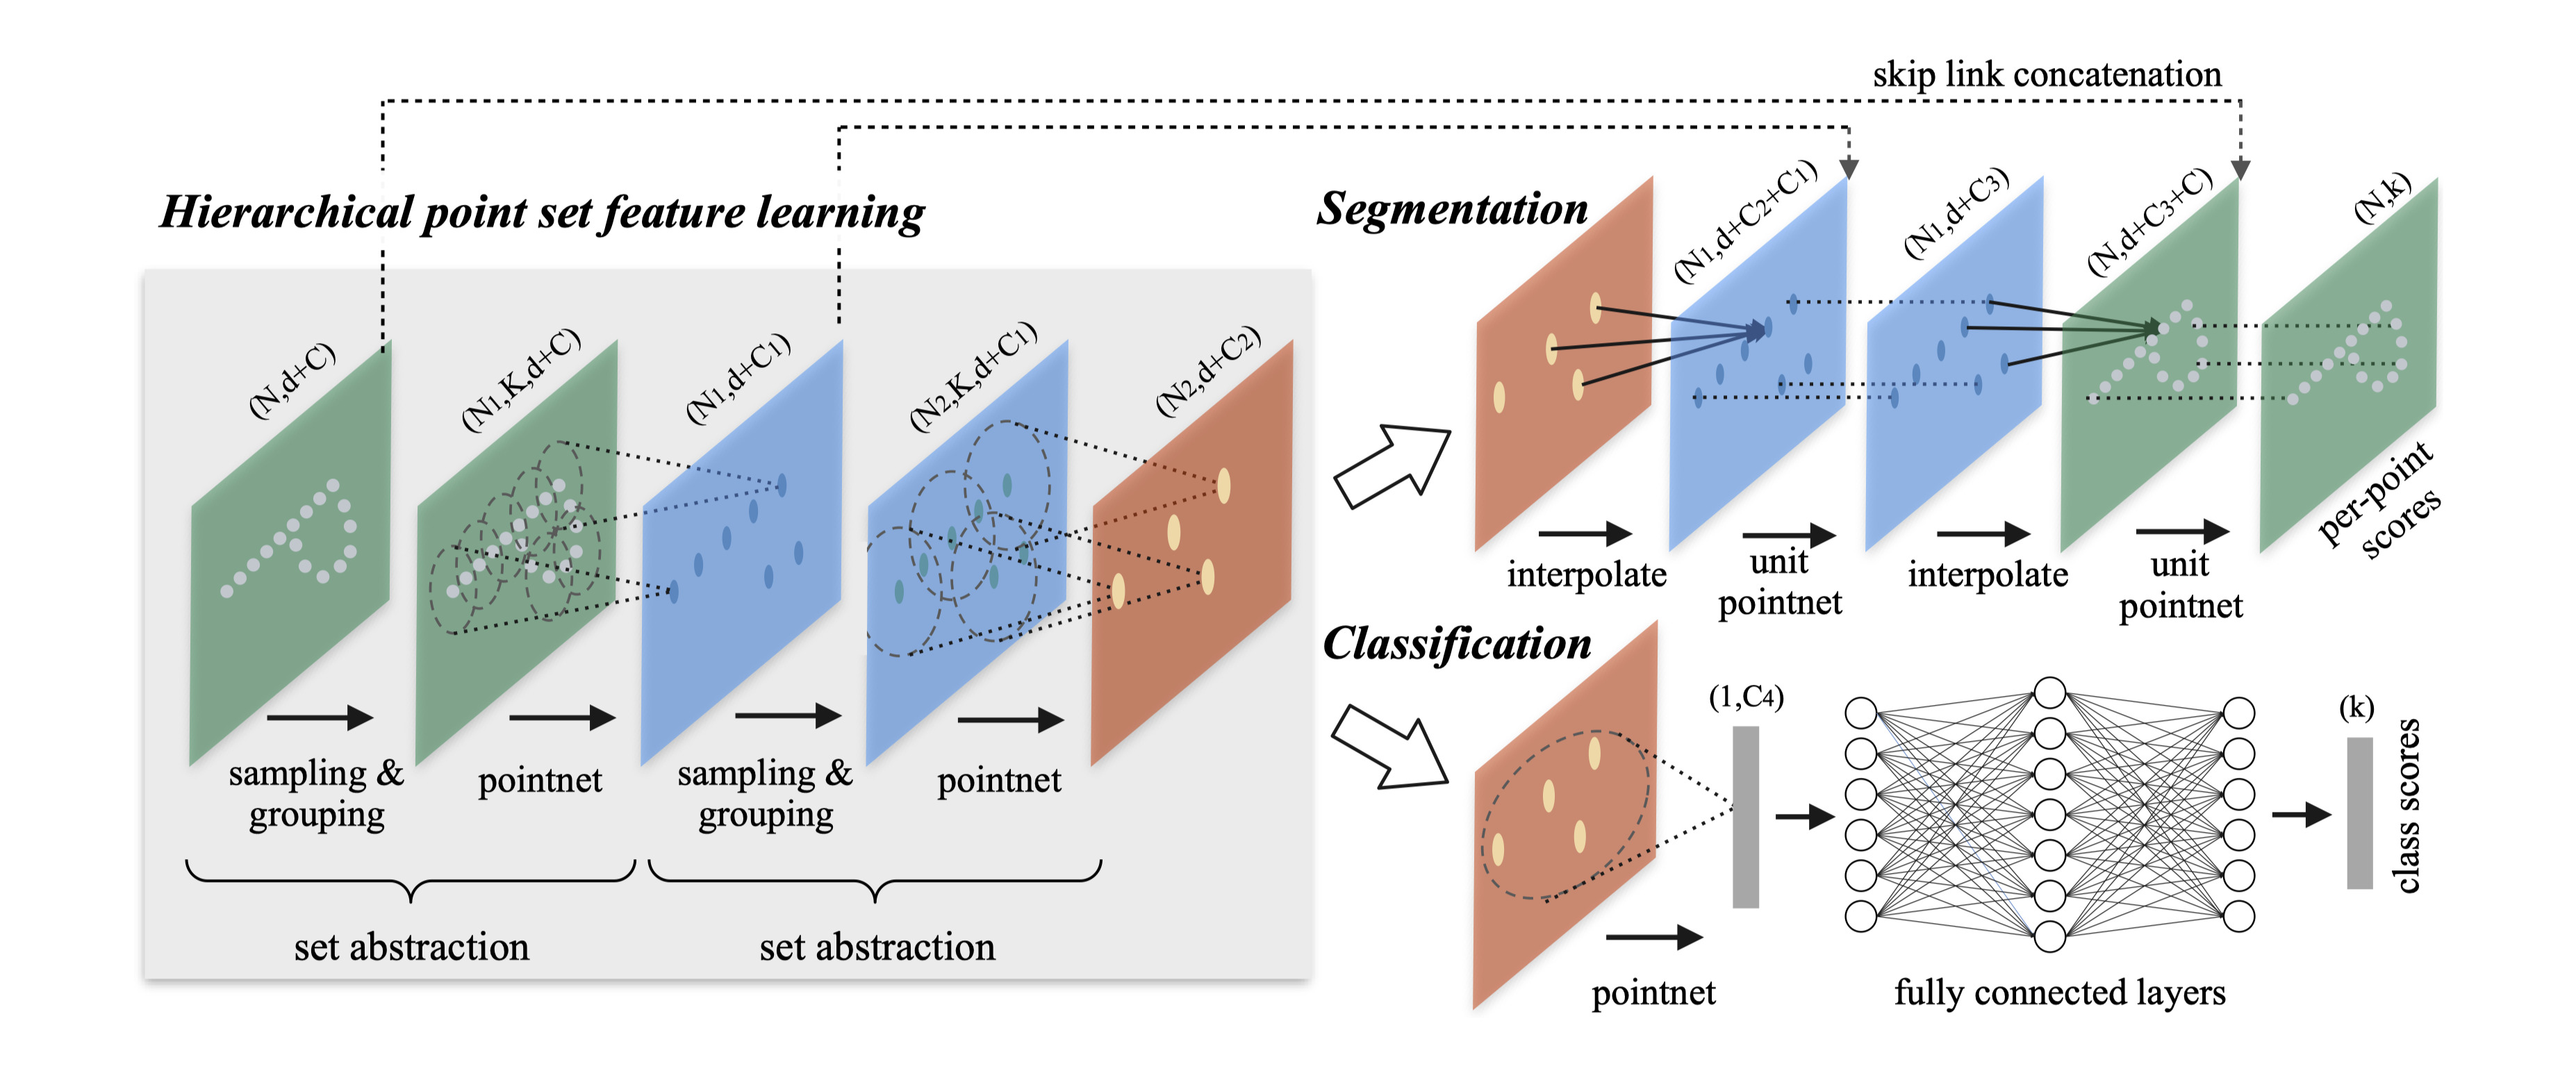
\includegraphics[width=\textwidth]{../images/pointnet2_architecture.jpg}
}
\caption[PointNet++ architecture]{\label{fig-pointnet2-architecture}PointNet++ architecture.
Figure from (Qi, Yi, et al. 2017)}
\end{figure}

\section{Area-based approach}\label{sec-area-based-approach}

The most common way to use \gls{lidar} for mapping forest attributes is the \gls{aba} \citep{whiteABAGuide2013}.
Figure~\ref{fig-aba-schema} shows its schematic representation.
It consists of a \gls{lidar} survey covering the whole area of interest and a manual forest inventory providing ground truth data for fitting statistical models and validating the results.
The inventory usually consists of many circular ground plots with every tree within counted and attributes of interest either directly measured or calculated and averaged.
The point cloud is clipped by the extents of the ground plots, and for each plot it is reduced to a collection of manually selected metrics.
The metrics usually include descriptions of the height distribution of the points, but often reflection intensities and other sensor-provided information is used as well, such as the return number, the number of returns, etc. (a brief discussion on the use of intensity-based features can be found in Section~\ref{sec-intensity-based-features}).
In general, any summary statistic that can be derived from a collection of points can be used, including features mentioned in Section~\ref{sec-ml-dl}.
These metrics are then used as input features for fitting regression and classification models to predict the forest attributes measured on the corresponding plots.
The same metrics are calculated for the entire area of interest, using a grid with a cell size similar in area to the area of a single ground plot.
The models are then applied to the grid, generating an extrapolation of the required attributes.

\begin{figure}
\centering{
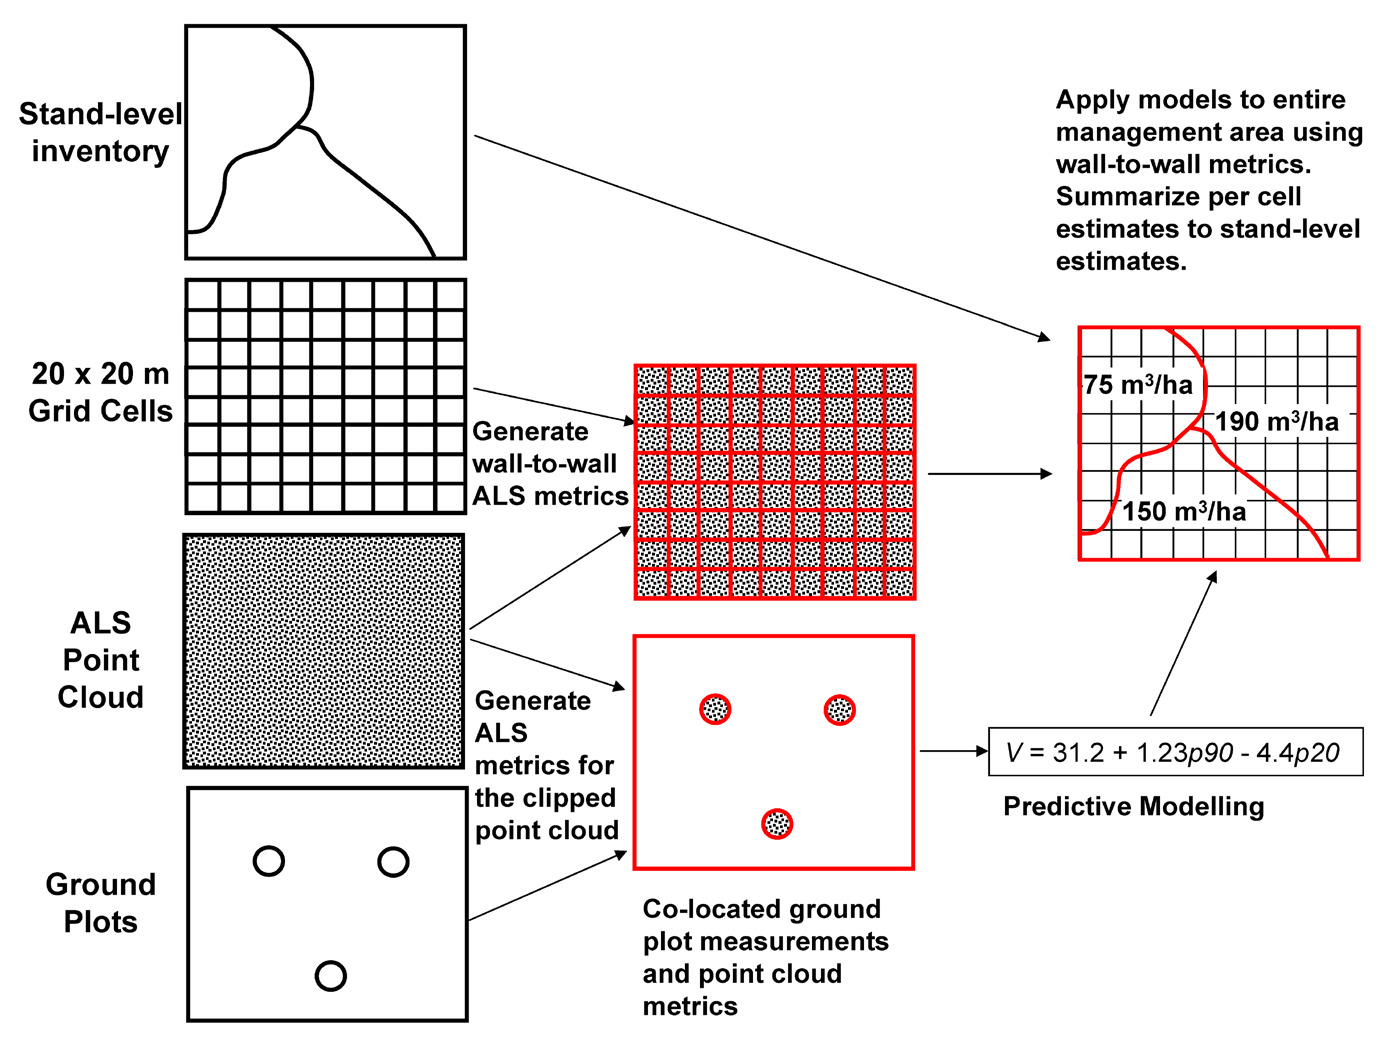
\includegraphics[width=\textwidth]{../images/aba_schematic.jpg}
}
\caption[Area-based approach schematic]{\label{fig-aba-schema}Area-based approach schematic. Figure
from (White et al. 2013)}
\end{figure}

Area-based approach is extensively used both in research and in industry because it provides many advantages.
It is relatively easy to implement.
In fact, basic familiarity with the R programming language is enough to create your own area-based approach pipelines since a full, scalable implementation exists in the \texttt{lidR} package \citep{rousselLidRPackage2020}.
It is also straightforward to extend with other data sources such as satellite or aerial images, and it works even with sparse data: for successful plot and stand level modeling point densities as low as 0.5 points per square meter have been reported to be enough [\citet{treitzLiDARSamplingDensity2012}; \citet{jakubowskiTradeoffsLidarPulse2013}].
Still, it requires a lot of field inventory data to work, since every ground plot becomes a single example for the models.
The models that can be used are also relatively simple, because of how expensive the data collection is.
Data-hungry approaches like neural networks usually do not have enough data to train.
The results are also very coarse – predicted on a grid with the size defined by the area of a plot (a common plot shape is a circle with 9-meter radius, which is approximately equivalent to a square grid cell with 16-meter side).
This is why they are usually further aggregated to stand level.

\subsection{Examples of studies using ABA}

As mentioned, area-based approach is used widely both throughout industry and research.
I have personally taken part in a couple of projects where it was used for mapping forest attributes on large scales.
This subsection offers some examples of its continuing use in research.

\citet{bouvierGeneralizingPredictiveModels2015} suggest a set of 4 metrics they use to fit models for predicting timber volume, above ground biomass, and basal-area on stand level, instead of most commonly used metrics based on the distribution of height.
Their metrics are aimed to capture different aspects of the canopy geometry.
The authors argue that usage of a very limited set of carefully engineered diverse metrics results in improvement of model generalization ability without loss of accuracy.

\citet{zhangImprovedAreabasedApproach2023} use a modification of the area-based approach to predict plot-level \gls{dbh} by utilizing known allometric dependencies between tree height and \gls{dbh} to limit the size of the hypothesis set for fitting regression models.
They use airborne \gls{lidar} measurements with an average density of 9.6 points per square meter and report a relative error of 11%.

\citet{vermeerLidarbasedNorwegianTree2023} use a U-Net \citep{ronnebergerUNetConvolutionalNetworks2015} image semantic segmentation model on \gls{lidar}-derived 1-meter resolution digital terrain models and canopy height maps to predict the distribution of three main tree species in a Norwegian forest.
They achieve a macro $F_1$ of 0.70 when including the background class, and 0.63 when including only the target species classes, as evaluated on independent field inventory plots.

\citet{kcEstimationAboveGroundForest2024} is a classic example of an area-based approach study utilizing airborne \gls{lidar} survey to predict forest above ground biomass.
They use a set of 32 metrics derived from height distribution of points, an automatic feature selection procedure, and two regression models: linear regression and Random Forest to compare the results.
They report coefficients of determination of 0.85 and average errors around 83 tons per hectare.


\section{Individual tree-based approach}\label{sec-individual-tree-approach}

With the constant improvement of accessibility and quality of high-resolution remote sensing data, there is a growing interest in the development of methods that operate on the scale of individual trees.
This subsection gives an overview of some of the research in this area, split by the main data source.

\citet{liNewMethodSegmenting2012} developed a well performing algorithmic method for segmentation of individual tree crowns in \gls{lidar} point clouds for coniferous forests that relies on the point shape characteristic of many coniferous species and segments the trees from top to bottom.

\citet{lucasIdentificationLinearVegetation2019} use the set of eigenvalue-based features calculated for each point in a fixed-radius neighborhood, with other geometrical features including maximum local height difference and height standard deviation, local radius and local point density, to identify linear vegetation elements in segmented point clouds.
They also use two point-based features that do not rely on a neighborhood: the number of returns and the normalized return number, proposed in \citet{guoRelevanceAirborneLidar2011}, and use Random Forest classifier to separate the points that belong to vegetation after first removing the planar features corresponding to grass, soil, and water surfaces.
The approach is somewhere in the middle between the area-based and individual tree-based, but still is a useful example of application of classic machine learning to segment out vegetation from larger point clouds.

\subsection{Image-only}

Many approaches rely only on images, mostly high-resolution \gls{rgb} and multispectral ones, but lately also hyperspectral.
The main advantage of such approaches is a well-established and well-known toolbox in terms of both algorithmic processing and deep learning, as many of the most important deep learning milestones were achieved in the field of computer vision.
They also can rely on consistent resolution, capture of fine details and textures, and continuous representation of sensed environments.
The main disadvantages were mentioned in the introduction: passive sensors rely on the sun as the source, and thus greatly depend on lighting such as cloud and terrain shadows, time of day, season.
They also offer no information on vertical structure.
Still, they are very popular and achieve outstanding results in many environments.

\citet{weinsteinDeepForestPythonPackage2020} introduces a Python package for training and inference of ecological object detection neural networks in airborne imagery.
It uses a convolutional object detection network described in \citet{weinsteinIndividualTreeCrownDetection2019} to predict bounding boxes for individual trees.
The data the model is trained on is not as dense as the forests that are the target of this thesis.
Moreover, the model requires fine-tuning to be applicable to new data, which greatly limits its applicability, since developing bounding box annotations for individual trees within dense forests is an extremely tedious and labor-intensive task.

\citet{lassalleDeepLearningbasedIndividual2022} use high-resolution satellite imagery to delineate individual tree crowns in mangrove forests by using DeepLabv3+-based Multi-Task Encoder-Decoder network (MT-EDv3), originally proposed by \citet{larosaMultitaskFullyConvolutional2021}, to predict for each pixel the distance to the tree crown border.
This distance map is then enhanced by applying the Laplacian over Gaussian filter, and finally the watershed segmentation algorithm is applied to delineate individual crowns.
The approach seems to rely on there being semi-clear separation between the tree crowns, which is rarely the case when the forests are dense and mixed.

The same network was also successfully used to map tree species in tropical urban environment in Rio de Janeiro, Brazil in \citet{martinsDeepLearningbasedTree2021}.
They develop a post-processing approach to combine the semantic segmentation map and the distance map to classify tree species with an average $F_1$-score of 79.3\% and resulting in a realistic tree species map.

\citet{oscoConvolutionalNeuralNetwork2020} use a convolutional neural network on \gls{uav} multispectral images to count citrus trees in an orchard by predicting a confidence map that shows the likelihood of each pixel containing a tree.
They report $F_1$-scores of up to 0.95, which is impressive even for managed stands.

\citet{venturaIndividualTreeDetection2024} describe a network they call HR-SFAnet, consisting of a VGG-16 \citep{simonyanVeryDeepConvolutional2014} backbone feature extractor, a confidence head, and a parallel attention head, for detecting individual trees in urban environments using high-resolution multispectral images.
The network is a deeper modification of the SFANet proposed in \citet{zhuDualPathMultiScale2019} for counting the number of people in photos.
They report $F_1$-scores of 0.75, with average positioning error of 2.2 meters.


\subsection{Terrestrial LiDAR}

Terrestrial \gls{lidar} surveys usually provide very dense and detailed point clouds.
Most importantly for the task of localizing individual trees, terrestrial measurements always capture the trunks of the trees clearly.
Tree trunks are very useful for tree detection and segmentation, and there are many algorithms that use bottom-to-top approaches that trace the trunks into the canopies.

\citet{burtExtractingIndividualTrees2018} introduce \texttt{treeseg}, a software package written in C++ for extracting individual trees from \gls{lidar} point clouds.
Even though it is designed and presented as a platform-agnostic method made to operate on both terrestrial and \gls{uav} \gls{lidar} point clouds, it relies on trunk detection, which is common for many methods based on terrestrial \gls{lidar} and often is not applicable to \gls{uav} \gls{lidar} data.

\citet{lopezserranoArtificialIntelligencebasedSoftware2022} introduce another software package called \texttt{AID-FOREST} for fully automatic processing of terrestrial \gls{lidar} point clouds based on trunk detection.
The software takes in a raw point cloud, performs all required preprocessing steps, and runs an object detection neural network on a series of horizontal slices to find cross-sections of trunks, and then processes the detection results from each level to track individual trees.

\citet{allenTreeSpeciesClassification2022} describe an approach for classifying terrestrial \gls{lidar} point clouds of individual trees extracted by \texttt{treeseg} using multi-view representation based on \citet{goyalRevisitingPointCloud2021} and a convolutional ResNet network \citep{heDeepResidualLearning2016}.
They report high classification accuracies both overall and per-species on a dataset of almost 2500 individual trees.

\citet{wilkesTLS2treesScalableTree2023} introduce \texttt{TLS2trees}, another automated framework for segmentation of individual trees in terrestrial \gls{lidar} point clouds, consisting of a set of Python command line tools.
The framework consists of three steps: preprocessing, semantic segmentation, and instance segmentation into a set of individual trees.
After that, a set of attributes are computed for each tree.
The software is designed to be horizontally scalable (meaning it's easy to speed up calculations by using more machines doing them in parallel, as opposed to vertically, meaning by increasing the computational resources available to a single machine) to address huge datasets produced during terrestrial laser scanning surveys.

All these software packages are impressive, but non-applicable to the data described in this work.

\citet{vianaTimberVolumeEstimation2022} use a small dataset to compare tree-level inventory metrics extracted from a terrestrial \gls{lidar} survey and from a manual inventory.
They report very good results, showing that terrestrial \gls{lidar} can serve as a replacement for manual inventories in diverse secondary forests (secondary forests are forests that regenerate naturally after significant disturbances like logging, storms, or fires).

\citet{nurunnabiDevelopmentPreciseTree2024} offer a compelling example of how detailed terrestrial \gls{lidar} point clouds can be used to provide very detailed analyses on tree level.
The authors report high accuracies on the task of segmenting the point clouds into wood and leaf points by utilizing geometric features mentioned earlier to locate linear and non-linear areas.
They then apply an octree-based segmentation algorithm to develop a precise 3D structure of a tree.

\subsection{UAV LiDAR}

A common approach to utilize \gls{lidar} point cloud data for tree detection is by calculating \glspl{chm} – images where each pixel represents the height of vegetation – and applying the same techniques as for image-only approaches.

A substantial number of different tree detection algorithms are variations of the local maxima filter, differing in what the filter is applied to, how many times, with what windows, and how the results are combined or preprocessed.
For example, \citet{doussExtractionIndividualTrees2022} offers an exploration of how different window size functions for the local maxima filtering applied to \gls{lidar}-derived canopy height maps affect the quality of individual tree detection.
They show that for a moderately dense forest in France, it is possible to find the parameters for the local maxima filter window that produce satisfactory results.
It is, however, clear that it requires great deal of manual adjustment, and visual inspection of the results of detection makes it clear that they are only locally consistent.
Any change in the canopy structure patterns noticeably affects the quality of the detection even for sophisticated window functions.

\citet{lisiewiczCorrectingResultsCHMBased2022} propose a way to improve the results of canopy height map-based individual tree segmentation algorithms.
Their approach consists of three steps.
The first step is the classification of segments into correct, under-segmented, or over-segmented using a Random Forest classifier, the second step is the refinement of under-segmentation errors by re-segmenting them with adjusted parameters, and the last step is the refinement of over-segmentation errors by merging with the correct segments using an algorithmic approach based on a collection of intensity-derived features.
The authors suggest that this approach is universal in terms of forest composition and complexity, unlike many other ad-hoc correction methods based on the study area and thus non-generalizable.

\citet{wangAutomaticDetectionIndividual2023} propose a two-stage network they call Tree \gls{rcnn} to detect trees in \gls{uav} \gls{lidar} point clouds.
The first step is generation of dense anchors across the point cloud that are then processed by the \gls{rcnn} to generate proposals for individual tree locations.
The second step involves multi-position feature extraction to refine the proposals.
The approach is evaluated on the NewFor benchmark \citep{eysnAlpineITDBenchmark2015} and outperforms all benchmark methods that come with it.

\citet{fuIndividualTreeSegmentationUAV2024} propose a method for segmenting individual trees in \gls{uav} \gls{lidar} point clouds based on a multiscale adaptive local maximum filter applied to the smoothed canopy height map to detect tree tops, a region-growing method for crown delineation that are then refined by a voxel-based clustering algorithm.
The method is developed and tested on 21 synthetic plots and one actual survey, and the authors report good accuracy for estimation of both tree locations and heights.
Worth noting that both the synthetic and real forest have relatively well-defined an unambiguous canopy structure.

\subsection{Fusion of data}

Many works do not just use one data source and instead combine multiple complimentary ones for better representation.
This subsection gives an overview of data fusion approaches for forestry applications on individual tree scale.

\citet{lianBiomassCalculationsIndividual2022} describe an approach for calculating individual tree biomass by combining \gls{uav} multispectral, \gls{uav} \gls{lidar} and terrestrial \gls{lidar} data.
Terrestrial and \gls{uav} \gls{lidar} are merged to get a more representative point cloud, showing the trees equally well both from above and from the ground.
The multispectral image is used to generate a species classification map, which is then used to segment the point cloud.
The segmented cloud is then used to estimate diameter at breast height and height and calculate above ground biomass.

\citet{liFusionApproachesIndividual2023} explore the contributions of multispectral images, very high resolution panchromatic images, and \gls{lidar} data during fusion on feature and decision level for tree species classification using Support Vector Machine and Random Forest classifiers on manually delineated tree crowns from an urban environment.
They report that fusion consistently improves the results over using each of the data sources on its own.
They also report that fusion on decision level resulted in the highest overall accuracy metrics.

\citet{balestraLiDARDataFusion2024} offers a review of 151 publications concerning fusion of \gls{lidar} data with other remote sensing data.
The authors report that in most cases fusion improves the results.
Most relevant to this thesis, they report that for individual tree segmentation the results of fusion-based approaches compared to \gls{lidar}-only ones are consistently better.
\citet{laExtractionIndividualTree2015} show an increase from 63\% to 92\% for low-density forests, and from 62\% to 70\% for high-density forests, \citet{aubry-kientzMultisensorDataFusion2021} show and improvement by 5\%, and \citet{zhenImpactTreeOrientedGrowth2014} and \citet{arenas-corralizaAutomaticMappingTree2020} improved their results by 2-4\%.

\citet{ferreiraImprovingUrbanTree2024} use a U-Net semantic segmentation model for fusion of \gls{vnir} images and airborne \gls{lidar}-derived feature maps including surface normals of the canopies, reflection intensities, canopy heights, and leaf-area index for mapping tree species in urban tropical areas.
Their results show that adding \gls{lidar}-based features improves $F_1$-scores across all considered species, with average $F_1$-score 84.1.
They also use the segment anything model \citep{Kirillov_2023_ICCV} to automatically segment tree crowns with outstanding 98\% boundary $F_1$-score.

\citet{wuFineClassificationUrban2024} use a combination of high-resolution \gls{rgb} images and \gls{lidar} to classify urban tree species by extracting seven different feature types and using a Random Forest for pixel-level classification.
They report on seven experiments using different combinations of extracted features.
The results show an improvement of 18.5\% in accuracy when using fusion of \gls{lidar} and \gls{rgb} compared to \gls{rgb}-only.


\subsection{Summary}

There is a lot of research going on currently on individual tree-level inventories using \gls{uav} remote sensing data.
Most results that can be considered successful are either in more mild environments, such as urban or managed forests, in predominantly coniferous forests, or use a much more detailed, but at the same time much more labor-intensive data source – terrestrial \gls{lidar}.
Mild forest types usually have canopy structures that are a lot easier to interpret, since the trees often stand far enough apart to be separable.
At the same time, they allow for much more signal penetration, resulting in a good representation of tree trunks in the data, which is tremendously useful for the task of detecting trees.
Predominantly coniferous forests, even dense ones, also have a canopy structure that is easy to interpret because conifer trees have a characteristic triangle shape that results in spikes in canopy height even when trees are standing close to each other.
Terrestrial \gls{lidar} data is different from \gls{uav} \gls{lidar} in the amount of detail and, most importantly, the perspective.
It surveys the trees from below, virtually guaranteeing the presence of trunks in the point clouds.
Several fully automated approaches to detailed forest inventories using terrestrial \gls{lidar} data exist that rely on the detection of trunks.
A gap persists in solutions that would consistently work on \gls{uav} remote sensing data over dense mixed forests, with complex overlapping canopies.
The active nature and the vertical structure information provided by \gls{lidar} is essential in such complex environments.
At the same time, many results indicate that fusion of \gls{lidar} point clouds with other data sources consistently improves the results in forestry applications, which is why the proposed framework relies on fusion of \gls{lidar} with \gls{rgb} imagery.
